%% 
%% Copyright 2007-2020 Elsevier Ltd
%% 
%% This file is part of the 'Elsarticle Bundle'.
%% ---------------------------------------------
%% 
%% It may be distributed under the conditions of the LaTeX Project Public
%% License, either version 1.2 of this license or (at your option) any
%% later version.  The latest version of this license is in
%%    http://www.latex-project.org/lppl.txt
%% and version 1.2 or later is part of all distributions of LaTeX
%% version 1999/12/01 or later.
%% 
%% The list of all files belonging to the 'Elsarticle Bundle' is
%% given in the file `manifest.txt'.
%% 
%% Template article for Elsevier's document class `elsarticle'
%% with harvard style bibliographic references

%\documentclass[preprint,12pt,authoryear]{elsarticle}

%% Use the option review to obtain double line spacing
%% \documentclass[authoryear,preprint,review,12pt]{elsarticle}

%% Use the options 1p,twocolumn; 3p; 3p,twocolumn; 5p; or 5p,twocolumn
%% for a journal layout:
%% \documentclass[final,1p,times,authoryear]{elsarticle}
%% \documentclass[final,1p,times,twocolumn,authoryear]{elsarticle}
%% \documentclass[final,3p,times,authoryear]{elsarticle}
%% \documentclass[final,3p,times,twocolumn,authoryear]{elsarticle}
%% \documentclass[final,5p,times,authoryear]{elsarticle}
 \documentclass[final,5p,times,twocolumn,authoryear]{elsarticle}

%% For including figures, graphicx.sty has been loaded in
%% elsarticle.cls. If you prefer to use the old commands
%% please give \usepackage{epsfig}

%% The amssymb package provides various useful mathematical symbols
\usepackage{amssymb}
\usepackage{lipsum}
%% The amsthm package provides extended theorem environments
%% \usepackage{amsthm}

%% The lineno packages adds line numbers. Start line numbering with
%% \begin{linenumbers}, end it with \end{linenumbers}. Or switch it on
%% for the whole article with \linenumbers.
%% \usepackage{lineno}

\usepackage{graphicx} % Required for inserting images
\usepackage{amssymb}
\usepackage{stfloats}
\usepackage{lipsum}  
\usepackage{todonotes}
\usepackage{appendix}
\usepackage{float}   
\usepackage{subfigure}
\usepackage{subcaption}
\usepackage{listings}
\usepackage{amsmath}
\usepackage{xurl}
\usepackage{caption}
\usepackage{booktabs}
\usepackage{multirow}
\usepackage{mathtools}
\usepackage{biblatex}
\usepackage{svg}
\usepackage{tikz}
\usepackage{quantikz}
\addbibresource{report.bib}
\usepackage{hyperref}
\usetikzlibrary{angles, quotes, 3d}
\usepackage{pgfplots}
\usepackage[dvipsnames]{xcolor}
\pgfplotsset{compat=1.18}
% \DeclarePairedDelimiter\bra{\langle}{\rvert}
% \DeclarePairedDelimiter\ket{\lvert}{\rangle}


% ------------------
% For figures
\usetikzlibrary {arrows.meta,bending,positioning} 

\usetikzlibrary{shapes.geometric, shapes.arrows}
\usetikzlibrary{patterns}
\usetikzlibrary{quantikz2}
     \tikzset{operator/.append style={fill=white!0}}
 % ----------

%% You might want to define your own abbreviated commands for common used terms, e.g.:
\newcommand{\kms}{km\,s$^{-1}$}
\newcommand{\msun}{$M_\odot}

%\journal{Results in Physics}

\makeatletter % Remove date and submitted to elsevier in foottext
\def\ps@pprintTitle{%
 \let\@oddhead\@empty
 \let\@evenhead\@empty
 \let\@oddfoot\@empty
 \let\@evenfoot\@empty
}
\makeatother

\begin{document}

\begin{frontmatter}

%% Title, authors and addresses

%% use the tnoteref command within \title for footnotes;
%% use the tnotetext command for theassociated footnote;
%% use the fnref command within \author or \affiliation for footnotes;
%% use the fntext command for theassociated footnote;
%% use the corref command within \author for corresponding author footnotes;
%% use the cortext command for theassociated footnote;
%% use the ead command for the email address,
%% and the form \ead[url] for the home page:
%% \title{Title\tnoteref{label1}}
%% \tnotetext[label1]{}
%% \author{Name\corref{cor1}\fnref{label2}}
%% \ead{email address}
%% \ead[url]{home page}
%% \fntext[label2]{}
%% \cortext[cor1]{}
%% \affiliation{organization={},
%%            addressline={}, 
%%            city={},
%%            postcode={}, 
%%            state={},
%%            country={}}
%% \fntext[label3]{}

% \title{\textbf{Mens Erger Je Niet With A Quantum Twist}\\
% \textbf{Introducing quantum effects by playing a quantum version of a board game}\\
% Creating a quantum board game (Mens erger je niet!) which can be run on a quantum computer to showcase quantum phenomena}
% From dice to qubits: A quantum version of Mens Erger Je Niet!
% Quantum Mens Erger Je Niet!: A Board Game to Demonstrate Quantum Mechanics that can be run on Quantum computer
%Creating a quantum board game to showcase quantum phenomena which can be run on a quantum computer
\title{Quantum "Mens Erger Je Niet!": A Board Game to Demonstrate Quantum Mechanics that can be run on a Quantum Computer}

%% use optional labels to link authors explicitly to addresses:
%% \author[label1,label2]{}
%% \affiliation[label1]{organization={},
%%             addressline={},
%%             city={},
%%             postcode={},
%%             state={},
%%             country={}}
%%
%% \affiliation[label2]{organization={},
%%             addressline={},
%%             city={},
%%             postcode={},
%%             state={},
%%             country={}}

\author[first]{Kyrian Rahimatulla, Alexis Fimeyer, Emirhan Balban, Guo Chuen Liu, Sjoerd Terlouw}
\affiliation[first]{organization={Delft University of Technology}}

\begin{abstract}
A quantum board game is constructed using the classical board game "Mens erger je niet!" as a foundation. New game mechanics are added and the size of the game is reduced. The positions on the board and the winning positions are encoded using qubits. As moves are made, classical logic is used to update the quantum circuit by appending quantum gates. Four bases are used to measure the positions of the pawns. With these bases, the Bell test is recreated. The quantum circuit is optimized to remove unnecessary gates and idle qubits to remain under the 29-qubit limit. The smaller circuit is then transpiled and run on the IBM Sherbrooke quantum computer and a simulator. It is concluded that superposition, entanglement and measurement can be implemented into the game while keeping it playable for the general audience as an educational resource.
\end{abstract}

%%Graphical abstract
%\begin{graphicalabstract}
%\includegraphics{grabs}
%\end{graphicalabstract}

%%Research highlights
%\begin{highlights}
%\item Research highlight 1
%\item Research highlight 2
%\end{highlights}

\begin{keyword}
%% keywords here, in the form: keyword \sep keyword, up to a maximum of 6 keywords
Quantum game \sep Mens erger je niet! \sep quantum mechanics \sep quantum gates \sep qubits

%% PACS codes here, in the form: \PACS code \sep code

%% MSC codes here, in the form: \MSC code \sep code
%% or \MSC[2008] code \sep code (2000 is the default)

\end{keyword}


\end{frontmatter}

% \tableofcontents

%% \linenumbers

%% main text

\section{Introduction}
\label{introduction}

Quantum mechanics is a notoriously difficult topic to understand. Beyond the abundance of mathematics involved in the field, quantum mechanics describes phenomena that are fundamentally different from the macroscopic classical phenomena that humans are intuitively accustomed to. Things like quantum superposition and entanglement are typically not observed at human scales. This poses a challenge for quantum mechanics education, as students not only need to master the mathematics but also reshape their intuition about how the world works physically. To this end, numerous games have been developed that claim to make players accustomed to quantum phenomena, like superposition, entanglement, interference, and collapse, by incorporating them into the mechanics of the game. Tic-Tac-Toe \cite{10.1119/1.2213635}, Minesweeper \cite{Quantum_Minesweeper}, Minecraft, Chess \cite{Akl2010OnTI, cantwell2019quantumchessdevelopingmathematical}, and Checkers have all gotten this treatment. \\
In quantum Tic-Tac-Toe the players can place marks in superpositions, such that a square can be occupied by several marks. At a certain point, the board collapses and a player has won or the game continues.  The game, however, is not very complex and does not show actual quantum mechanics, since it can be played on paper. Quantum minesweeper consists of several minesweeper boards in superposition. The player performs different types of measurements to try and guess the superposition. Unfortunately, the game only shows superposition, entanglement and collapse, of which the last one is the only one that is influenced by the player. \\  
Some of these games, as previously mentioned, like Quantum Tic Tac Toe and Quantum Minecraft, are not meant to be run on a quantum computer. Quantum Checkers and Cantwell's Quantum Chess are designed with quantum circuits in mind, but the practical considerations of running them on today's QPUs have not been taken into account. These games succeed to varying degrees at demonstrating superposition, entanglement, interference, and collapse. There is, however, one missing piece in this puzzle: what happens when different measurement bases are used? Measuring in different bases is typically used to demonstrate the fundamental difference between quantum and classical uncertainty, like in the Bell test \cite{BellSecond, BellOriginal}, but no quantum board games were found that implemented this feature. The goal of this project is to create a quantum version of the German board game Mensch Ärgere Dich Nicht!\footnote{If you are unfamiliar with this game, see the quick introduction on Wikipedia \url{https://en.wikipedia.org/wiki/Mensch_\%C3\%A4rgere_Dich_nicht}} that demonstrates superposition, entanglement, and measurement in different bases, and can actually be run on a quantum computer and simulator. This goal will be achieved using the Python package Qiskit \cite{qiskit2024}. Then, it will be shown that this game is capable of replicating the Bell test.

\section{Method and Results}\label{Main}
\subsection{Quantum Mens erger je niet! and its mechanics}\label{GameMechanics}
In the quantum version, players do not throw one, but two dice when moving a pawn. The pawn moves forward by the value of each individual die simultaneously. Thus, the pawn is then in a superposition of having moved forward by different values, that both have half of the original probability. In the second turn, the player selects one of the two superpositions to split up further again. This way the number $N$ of positions of a single pawn with $s$ splits is given by $N = 1 + s$. It is also possible that players throw the same value twice; in that case, the pawn that moves forward does not split into two new positions and is moved just like in a classical game. The movement described above also works for pawns that are already in a superposition of different positions. 

When a pawn, possibly in a superposition, lands on another pawn of a different colour (which can also be in a superposition), a capture is registered. The first pawn is called the \textbf{capturer} and the second pawn is called the \textbf{captive}. Since the pawns can be in a superposition, the captive could be captured and at the same time not be captured. Now there are two different pawns occupying the same tile. However, as explained in Section \ref{quantum_circuit}, each position has only one qubit associated with it, where the up state means free, and the down state means occupied. Therefore, measuring the circuit can not reveal which pawn occupies that spot. To avoid this problem, a new rule is introduced called the \textbf{no-double-occupancy rule} \cite{cantwell2019quantumchessdevelopingmathematical}, which states that each position can only be occupied by a single pawn. During a capture move, the capturer becomes entangled with the captive, but the captive is not removed from the board. The capturer then lands on the next free spot in front of the captive, to satisfy the no-double-occupancy rule.  All possible moves and the rules associated with them are given in \ref{app:ExampleMoves}. \\

% Introduce the side effect and measures to counteract them. 

In the classical game, pawns can overshoot their winning space and move backwards, but in the quantum version, backwards movement is impossible. When a pawn sets foot in its winning space, a measurement will occur regardless of the moves remaining. If after measuring the pawn is indeed inside the winning space, then it will occupy the remaining free spot in the winning space. Another way a measurement can occur is when more than twenty pawns are on the board. A measurement must occur when this condition is met to stay below the 29-qubit limit, as the simulator only has access to 29 qubits. For $m$ filled positions, roughly $m$ qubits are needed, but with entanglement, the final number of qubits needed can be higher. Besides this, the limit is also set to make the game more clear. After a measurement, all superpositions will collapse and only after a measurement captured pawns can be removed from the board. 
\\
So, there are two situations which can cause a measurement to occur. When the measurement is triggered by exceeding the twenty positions limit, all the qubits are measured in the standard basis. In the other case, the four players are measured in different bases. There are four bases used for measurement. These are the Z-basis, X-basis, Q-basis and R-basis. The Z-basis and X-basis are already well known, while the Q-basis and R-basis are newly defined bases. Measurement in different bases is achieved by adding a gate in front of a measurement in the $Z$-basis.  For each basis, one of the basis vectors represents a pawn being present, while the other vector is associated with the pawn not being present. This works in the same way as what $\ket{0}$ and $\ket{1}$ mean, where $\ket{0}$ means that no pawn is present and $\ket{1}$ means that there is a pawn present. 
% The basis vectors of the four bases are represented inside a Bloch sphere in Figure \ref{fig:BlochSphere}, from which it can be seen that the Q-basis consists of the diagonal going in between $\ket{0}$ and $\ket{+}$ and that the R-basis is the diagonal which goes in between $\ket{1}$ and $\ket{+}$. 

% \begin{figure}[H]
%     \begin{tikzpicture}
%       % Define radius
%       \def\r{3}
    
%       % Bloch vector
%       % \draw (0, 0) node[circle, fill, inner sep=1] (orig) {} -- (\r/3, \r/2) node[circle, fill, inner sep=0.7, label=above:$\vec{a}$] (a) {};
%       % \draw[dashed] (orig) -- (\r/3, -\r/5) node (phi) {} -- (a);
    
%       % Sphere
%       \draw (0, 0) circle (\r);
%       \draw[dashed] (0, 0) ellipse (\r{} and \r/3);
%       \draw[dashed] (0, 0) ellipse (\r/3 and \r{}); 
    
%       % Axes, here coordinates are of form (y, z, x)
%       \draw[green, line width = 0.5mm, ->] (0, 0, 0) -- ++(0, 0, 0.85 * \r) node[right, below] (x1) {\textcolor{black}{$\ket{+}$}};
%       \draw[green, line width = 0.5mm, dashed, ->] (0, 0, 0) -- ++(0, 0, -0.85 * \r) node[above, right] (x4) {\textcolor{black}{$\ket{-}$}};
%       \draw[blue, thick, ->] (0, 0, 0) -- ++(\r, 0, 0) node[below, pos=1.1] (x2) {\textcolor{black}{$\ket{+i}$}};
%       \draw[blue, thick, dashed, ->] (0, 0, 0) -- ++(-\r, 0, 0) node[left, below, pos = 1.1] (x5) {\textcolor{black}{$\ket{-i}$}};
%       \draw[red, line width = 0.5mm, ->] (0, 0, 0) -- ++(0, \r, 0) node[right, pos=1.1] (x3) {\textcolor{black}{$\ket{0}$}};
%       \draw[red, line width = 0.5mm, dashed, ->] (0, 0, 0) -- ++(0, -\r, 0) node[below] (x6) {\textcolor{black}{$\ket{1}$}};
    
%       % \draw[->] (0, 0) -- ++(-2*\r / 5, -2*\r/ 3) node[below] (x7) {\textbf{x}};
%       % \draw[->] (0, 0) -- ++(\r + 1, 0) node[right] (x8) {\textbf{y}};
%       % \draw[->] (0, 0) -- ++(0, \r) node[above] (x9) {\textbf{z}};

%       \draw[->] (0, 0, 0) -- ++(0, 0, 1.25 * \r) node[below] (x7) {\textbf{x}};
%       \draw[->] (0, 0, 0) -- ++(1.25 * \r, 0, 0) node[below] (x8) {\textbf{y}};
%       \draw[->] (0, 0, 0) -- ++(0, 1.25 * \r, 0) node[above] (x9) {\textbf{z}};

%       % Axes for the Q-Basis, (y, z, x)
%       \draw[thick,solid, cyan, ->] (0,0,0) -- (0,\r / 1.3,\r / 1.3) node[left]{$q_1$};
%       \draw[thick, dashed, cyan, ->] (0,0,0) -- (0, -\r / 1.3, -\r / 1.3) node[right]{$q_2$};
%       \draw[thick,solid,brown,->] (0,0,0) -- (0, -\r / 1.79, \r / 1.79) node[below]{$r_1$};
%       \draw[thick, dashed, brown, ->] (0,0,0) -- (0, \r /1.79, -\r / 1.79) node[right]{$r_2$};
%     \end{tikzpicture}
%     \caption{Bloch sphere, where the basis (unit) vectors for the Q-basis and R-basis are given by $q_i$ and $r_i$ respectively. Furthermore these basis vectors are all inside the x,z-plane.}
%     \label{fig:BlochSphere}
% \end{figure}

% To visualize the basis vectors in the Bloch sphere, the Bloch sphere representation can be used. It is similar to spherical coordinates, where $\theta$ is the polar angle and $\phi$ is the azimuthal angle. The general form of the representation is given by Equation \ref{BlochSphereRepresentation}.
% \begin{equation}
%     \ket{\psi} = \cos \left( {\frac{\theta}{2}} \right) \ket{0} + \exp{(i \phi)} \sin \left( {\frac{\theta}{2}} \right) \ket{1} \text{.}
%     \label{BlochSphereRepresentation}
% \end{equation}

% Using Equation \ref{BlochSphereRepresentation}, the basis vectors for the Q-basis and R-basis are described by
% \begin{align}
%     \begin{split}
%         \ket{q_1} = \cos \left( {\frac{\pi}{8}} \right) \ket{0} + \sin \left( {\frac{\pi}{8}} \right) \ket{1} \\
%         \ket{q_2} = \cos \left( {\frac{3 \pi}{8}} \right) \ket{0} + \exp{(i \pi)} \sin \left( {\frac{3 \pi}{8}} \right) \ket{1}
%     \end{split}
% \end{align}
% \begin{align}
% \begin{split}
%     \ket{r_1} = \cos \left( {\frac{3 \pi}{8}} \right) \ket{0} + \sin \left( {\frac{3 \pi}{8}} \right) \ket{1} \\
%     \ket{r_2} = \cos \left( {\frac{\pi}{8}} \right) \ket{0} + \exp{(i \pi)} \sin \left( {\frac{\pi}{8}} \right) \ket{1} \text{.}
% \end{split}
% \end{align}
% \\
The gates added in front of the Z-measurement are described by the following matrices in $\ket{0},\ket{1}$ notation:
\begin{align}
\begin{split}
    R(\theta)=\left[\begin{matrix} \cos(\theta/2) & -\sin(\theta/2) \\ \sin(\theta/2) & \cos(\theta/2) \\ \end{matrix}\right], \\
    \text{with } \theta=\pi/4 \text{ for the Q-basis} \\
    \text{and } \theta = 3\pi/4 \text{ for the R-basis}
\end{split}
\label{eq:Rtheta}
\end{align}
\begin{align}
\begin{split}
    H=\frac{1}{\sqrt{2}}\left[\begin{matrix}1 & 1 \\ 1 & -1 \\ \end{matrix}\right], \\
    \text{ for the X-basis} \\
\end{split}
\label{eq:Heq}
\end{align}
The Z-basis does of course not get a gate in front, since this is the basis that the system is measured in. Which colour gets measured in which basis, depends on the type of pawn that triggered the measurement and is given in Table \ref{tab:MeasureBasisonTrigger}. From Table \ref{tab:MeasureBasisonTrigger} it is clear that the colour which triggers the measurement is always measured in the Z-basis.

\begin{table}[H]
    \centering
    % \caption{Which colour gets measured in what basis depending on which pawn enters the winning space. Where Z, Q, X  and R stand for the Z-basis, Q-basis, X-basis and R-basis respectively.}
    \caption{The bases which are used to measure each colour, depending on the pawn that enters the winning space. Here Z, X, Q and R stand for the Z-basis, Q-basis, X-basis and R-basis respectively.}
    % FOR TABLES THE CAPTION SHOULD GO ABOVE 
    \begin{tabular}{|c|c|c|c|c|}
        \hline
        Pawn\textbackslash Basis  & Z & Q & X & R \\
        \hline
        Red 1 & \textcolor{red}{R} & \textcolor{green}{G} & \textcolor{blue}{B} & \textcolor{Mulberry}{P} \\ 
        \hline
        Red 2 & \textcolor{red}{R} & \textcolor{Mulberry}{P} & \textcolor{blue}{B} & \textcolor{green}{G} \\ 
        \hline
        Blue 1 & \textcolor{blue}{B} & \textcolor{Mulberry}{P} & \textcolor{red}{R} & \textcolor{green}{G} \\
        \hline
        Blue 2 & \textcolor{blue}{B} & \textcolor{green}{G} & \textcolor{red}{R} & \textcolor{Mulberry}{P} \\ 
        \hline
        Green 1 & \textcolor{green}{G} & \textcolor{red}{R} & \textcolor{Mulberry}{P} & \textcolor{blue}{B} \\
        \hline
        Green 2 & \textcolor{green}{G} & \textcolor{blue}{B} & \textcolor{Mulberry}{P} & \textcolor{red}{R}  \\ 
        \hline
        Purple 1 & \textcolor{Mulberry}{P} & \textcolor{blue}{B} & \textcolor{green}{G} & \textcolor{red}{R} \\ 
        \hline
        Purple 2 & \textcolor{Mulberry}{P} & \textcolor{red}{R} & \textcolor{green}{G} & \textcolor{blue}{B} \\
        \hline
    \end{tabular}
    \label{tab:MeasureBasisonTrigger}
\end{table}

% \begin{equation}
%     S = \langle A_1 \otimes B_1 \rangle - \langle A_1 \otimes B_2 \rangle + \langle A_2 \otimes B_1 \rangle + \langle A_2 \otimes B_2 \rangle
% \end{equation}

The results of measuring all the colours in the standard basis are relatively easy to understand. Superpositions collapse to a single position, and if a capturer collapses to a position coming from the capture position, the captive is removed from the board. But measuring each colour in different bases gives rise to two strange side effects, which makes the game less intuitive (and even more quantum). The first side effect is that capturing becomes a bit stranger: a captured pawn can be removed even if the capturer collapses into a position which did not originate from the capture position. In other cases, the captured pawn is not removed, even though the capturer has collapsed into a position which originated from the capture position. The second side effect is that the players might gain or lose pawns. Consider a pawn with $n$ points in its superposition. After measurement, it could happen that the pawn still occupies these $n$ positions, hence the player has gained pawns after measurement. In the other case, it could happen that all $n$ points have vanished and the pawn has thus disappeared from the board. 

If the second side effect is left ignored, then this could very quickly bloat the board with totally new pawns. This comes with all sorts of problems. A player can win without having all their pawns in their winning positions, the board fills up too quickly and it is confusing for players to have several of the same pawns.
Therefore whenever multiple positions of a pawn remain on the board after measurement, only the furthest pawn remains and the rest is discarded. The uncaptured pawns that have disappeared from the board after measuring return to their home base outside the board. \\

With the ability to measure in different bases, it is possible to recreate the Bell test while playing the game. To achieve this, one has to create a reduced board state in the following sequence:
\begin{enumerate}
  \item Start with $\ket{110010}$ with Green 1, Red 1 and Green 2 in the occupied positions respectively.
  \item  Then get $\frac{1}{\sqrt{2}}(\ket{101010} - \ket{100001})$:  Red 1 throws a 1 and a 3. This causes Red 1 and Green 2 to be entangled. 
  \item Finally $\frac{1}{\sqrt{2}}(\ket{000110} - \ket{000101})$: Green 1 throws double 3, so it captures Red 1.
\end{enumerate}

\begin{equation}
    \ket{\psi^-}=\frac{1}{\sqrt{2}}(\ket{10} - \ket{01})
    \label{eq:singlet_state}
\end{equation}

The last state can be separated into $\frac{1}{\sqrt{2}}(\ket{0001} \otimes (\ket{10} - \ket{01}))$, which is the Bell state shown in Equation \ref{eq:singlet_state}. By triggering a measurement with a pawn at the winning position, the Bell state will be measured in different bases. For example, if Purple 1 triggers the measurement, the measurement bases will be R for Red 1 and X for Green 2. The Bell inequality is as follows:
\begin{equation}
    |S| = |\langle A_{1} B_{1} \rangle - \langle A_{1} B_{2} \rangle + \langle A_{2} B_{1} \rangle + \langle A_{2} B_{2} \rangle|  \leq 2
    \text{.}
\end{equation}

By triggering the winning positions of Red 2 and Blue 2, the matrices become $A_{1} = Q, A_{2} = R, B_{1} = X$ and $ B_{2} = Z $, which can be seen from Table \ref{tab:MeasureBasisonTrigger}. This will replicate the Bell test as can be seen in Figure \ref{fig:bell_test_results}. \\
To calculate the expected value of $S$, the individual expectation values need to be calculated. In general, the expectation value is given by the following derivation: define $\mathbf{A_{i}}$ and $\mathbf{B_j}$ as the gates in front of the measurement for basis $\langle A_iB_j \rangle$. Which gates these exactly are, is given by Equation \ref{eq:Rtheta} and \ref{eq:Heq}. Now the state in question given by Equation \ref{eq:singlet_state} becomes becomes
\begin{equation}
|\psi_o \rangle = (\mathbf{A_{i}} \otimes \mathbf{B_j})\ket{\psi^-}
\end{equation}
The expectation in general is given by $\langle A \rangle = \operatorname{Tr}(\rho A)$, with $A$ as the observable and $\rho=|\psi \rangle \langle \psi |$. Since qiskit measures in the $Z$-basis, the expectation will become:
\begin{align}
    \begin{split}
        \langle A_i B_j \rangle = \operatorname{Tr}(\rho_o (Z\otimes Z)), \\
        \text{ with } \rho_o= (\mathbf{A_{i}} \otimes \mathbf{B_j})\ket{\psi^-}\bra{\psi^-}(\mathbf{A_{i}} \otimes \mathbf{B_j})^\dagger
    \end{split}
\end{align}
Evaluating this gives the following values\footnote{The calculation itself is tedious, but quite straightforward. It can be found on \url{https://github.com/SjdTl/QuantumEngineering/blob/main/Report/bells_inequality.ipynb}}:
\begin{align}
    \begin{split}
        \langle ZR \rangle = \langle XR \rangle = \langle XQ \rangle = \tfrac{1}{2}\sqrt{2} \\
        \langle ZQ \rangle = - \tfrac{1}{2} \sqrt{2}
    \end{split}
\end{align}
This then violates Bell's inequality exactly in the way that is found in the measurements described in figure \ref{fig:bell_test_results}:
\begin{equation}
    S=\langle ZR \rangle + \langle XR \rangle + \langle XQ \rangle - \langle ZQ \rangle = 2 \sqrt{2}
\end{equation}
% The interesting part of the figure is that it takes quite a while to reach the expectation value of $S$. This can be explained using the variance of $S$. The variance is given by $\langle A^2 \rangle =\operatorname{Tr} \rho A^2$. Calculating this for the system gives:
% \begin{equation}
%     \langle (ZR)^2 \rangle = \langle (XR)^2 \rangle = \langle (XQ)^2 \rangle = \langle (ZQ))^2 \rangle = 1
% \end{equation}
% So the variance for all the expectation values is $\sigma^2 = 1/2$. It will be quite hard to exactly relate this to the 
\begin{figure}
    \centering
    \includesvg[width=1\linewidth]{Figures/bell_test_results_edited}
    \caption{Results of running the bell test. The first few hundred runs show that the value of $S$ is very slowly approaching $2\sqrt{2}$.}
    \label{fig:bell_test_results}
\end{figure}

% \subsection{Difference between the classical board game}


Besides the obvious differences between the classical and quantum game by introducing quantum effects, the game setup has also been changed. First, the board size has been reduced from 40 to 32 positions and the total amount of pawns for each colour has been reduced from 4 to 2. The reason for this is to reduce the complexity and the number of qubits needed to encode the positions of the pawns, such that it can run on a (simulated) quantum chip. This is because real quantum chips have a limited runtime and the local simulator has a limitation of about 29 qubits. More information about these limitations can be found in Section \ref{sec:run_circuit}. 


\subsection{The quantum circuit}
\label{quantum_circuit}
\begin{figure*}[b!]
    \centering
    \includesvg[width=0.7\linewidth]{Figures/general_implementation.svg}
    \caption{Each position is represented by a qubit. With each move the quantum circuit is updated. In this case, the qubit $\ket{1}_2$ representing the first red pawn becomes a superposition $\ket{01}_{47}+\ket{10}_{47}$.}
    \label{fig:general_implementation}
\end{figure*}
Each qubit represents a position on the board. The state $\ket{1}$ represents an occupied spot and $\ket{0}$ an unoccupied spot. The positions of the board are therefore represented by $\ket{n_0} \otimes \ket{n_1} \otimes \dots \otimes \ket{n_{31}}$, with $n_i \in \{0, 1\}$ and $i \in \{0, \dots, 31\}$. Mainly due to this system, there is a no-double-occupancy rule: the qubits do not keep track of the colour or type of pawn and therefore would be unable to differentiate two pawns in superposition on the same spot.
After a throw, the classical code identifies the type of move. It then tells which gates to append to the quantum circuit for that type of move.
This process is shown in Figure \ref{fig:general_implementation}. Usually, these gates span three qubits, but with a capture, the gates usually span more qubits. More information on the specific gates used can be found in \ref{app:ExampleMoves}.

For the winning positions of the pawns, more qubits have to be added. These qubits work the same as the regular qubits, except that only two are required since each player moves at most one pawn into a superposition of two pawns when arriving at a winning position. Due to following this up with a measurement, the eight winning positions can share two qubits between them. 
\\
A naive implementation would perhaps even assume that this amount can be brought down to one qubit since moving into the final positions with a superposition is the same as swapping into the final positions. However, this does not take into account the possibility of one of the superpositions getting into the final positions while capturing another pawn at the same time. \\ \\
Another possibility is to couple several qubits to a pawn instead of coupling each qubit to a position. Then, each pawn has a binary representation of its position on the board. In practice, this would mean that if red's first pawn is on position 16, its associated qubits would be in $\ket{01000}$. This would require $n\log_2{N}=40$ qubits for $n=8$ pawns on a board of $N=32$ positions, instead of just $N=32$ qubits. The benefit of this method is that pawns could now occupy the same position, but at the cost of the implementation being less general; adding more pawns would increase the amount of necessary qubits way more instead of not influencing the amount of qubits. However, the main problem is that the gates are very complex and counter-intuitive. A standard move gate could span five qubits, and a capture up to ten qubits. 



\subsection{Running the circuit}\label{sec:run_circuit}
The circuit can be either simulated or executed on a real quantum chip. The simulation is performed locally using the Aersimulator \cite{qiskitAer2024}. In version 0.16, the simulator can handle up to 29 non-idle qubits with noise on our machine. However, it struggles with circuits that involve a lot of entanglement, but the limits for that scenario are more difficult to define.
To still be able to simulate the 34 qubits with noise, the circuit is first optimized to remove unnecessary gates and then the idle qubits are removed from the circuit. The new smaller circuit is then transpiled on a simulated IBM Sherbrooke backend and then simulated using the Aersimulator.\\
The game is run on the IBM Eagle quantum computing platform, which is the only platform from IBM that is available for free\footnote{See \url{https://quantum.ibm.com/services/resources}}. This platform, like all quantum computers that contain more than 51 qubits (as of 2024) \cite{cao2023generation}, does not have complete entanglement\footnote{The map of the entanglement can be found on the IBM website at \href{https://quantum.ibm.com/services/resources?system=ibm_sherbrooke}{IBM Sherbrooke}}, meaning that not every pair of qubits is entangled. In this implementation of Quantum Mens Erger Je Niet, entangled states between distant qubits are created liberally. This means that the generated circuit might try to entangle two qubits that can not be entangled. Fortunately, if the circuit is run on a QPU with a universal quantum gate set and enough qubits, it is always possible to remap the circuit to efficiently approximate it on the architecture \cite{kitaev1997quantum}. This remapping does not have to be programmed from scratch, as it is already integrated in the Qiskit transpiler. The Qiskit transpiler takes the quantum circuit generated by the gameplay and modifies its topology in such a way that the specified backend (in this case IBM Eagle) can compute it. The various QPUs implementing the Eagle platform have median qubit readout errors on the order of $10^{-2}$ \href{https://quantum.ibm.com/services/resources}{IBM QPUs}. Measures are implemented to reduce the effect of these errors. Whenever a measurement is triggered, the circuit is executed and measured $1024$ times. All outcomes that occur less than $0.2\%$ of the time are discarded. Then the final result is selected from the remaining outcomes, taking their frequency into account in a classical weighted random selection.


\section{Discussion}\label{discussion}
This quantum version of the classic “Mens Erger Je Niet!” game demonstrates that quantum-mechanical principles, such as superposition, entanglement, and measurement collapse can be successfully integrated into a board game while keeping its original playability. Implementing these quantum features required modifications to the rules, including the no-double-occupancy constraint and additional measurement and capture steps.

From a technical standpoint, encoding each position on the board as a single qubit gives a good balance between gate complexity and hardware limitations. This ensures that important phenomena like superposition and entanglement remain observable. At the same time, it shows trade-offs: the simplifications (such as reducing board size and the number of pawns) show the limited number of qubits and connectivity constraints in current quantum devices.

For further improvements, combining interference effects into the gameplay could showcase more quantum behaviours. Additionally, scalability remains a problem. Implementing richer configurations, potentially adding more pawns or a larger board, would require both hardware advances and algorithmic optimizations, such as more efficient gate placement and circuit transpilation.

Overall, this adaptation shows the potential of “gamified” approaches for exploring quantum mechanics. By showing phenomena that differ from classical intuition, such as superposition and entanglement. Players gain a sense of quantum mechanics’ unique features. Ongoing improvements in both hardware and circuit design will make increasingly more complex quantum board games feasible.

% TODO: Mention that we performed Bell test and from which is followed that game is indeed quantum
\section{Summary and conclusions}
%%\label{}
This paper presents a quantum adaptation of the board game "Mens Erger Je Niet!" as a tool to demonstrate and explore quantum phenomena such as superposition, entanglement, and measurement collapse. By incorporating quantum mechanics into familiar game mechanics, the game serves as a bridge to introduce these principles to a wider audience. Although the implementation shows the feasibility of integrating quantum logic into gameplay, it also shows the challenges of balancing playability with the complexity of quantum logic. 
% Further developments could focus on expanding the scope of quantum interactions, refining rule sets, and optimizing the game's compatibility with real quantum hardware to further enhance its value and accessibility. 
By performing the Bell test in game, it was proven that the game indeed follows quantum mechanical principles. The result of the Bell test is in line with what would be expected based on the theory.
Further developments could focus on expanding the scope of quantum interactions, refining rule sets, and optimizing the game's compatibility with real quantum hardware to further enhance its value and accessibility.


\section*{Acknowledgements}
We would like to thank Menno Veldhorst for organizing the course and providing guidance throughout this project. Our gratitude also extends to Anasua Chatterjee, Stefano Bosco and Giordano Scappucci for their valuable feedback and support during our meetings. Their insights have been essential to the development and completion of this report.

%% The Appendices part is started with the command \appendix;
%% appendix sections are then done as normal sections
\appendix

\section{Move circuits}\label{app:ExampleMoves}
Dedicating a whole section to explaining how a full game would play out, would become far too large as the game itself is rather complex. Instead, the five fundamental moves of which all possible moves consist out of are given. These moves are called swap, superposition move, new pawn, capture and measure. The type of move is detected using classical code, which then updates the UI and appends the corresponding quantum gates to the circuit.
In the figures, the pawn movement and the corresponding circuit is given. It is assumed that the move is started from a mostly ‘clean’ circuit. The different pawns are represented by the patterns inside the positions.

\subsection{New pawn}
The simplest move is adding a new pawn to the game. This move can be made when at least one of the dice is a 6. The circuit is updated by just adding an X-gate to the relevant qubit.
\begin{figure}[H]
    \centering
    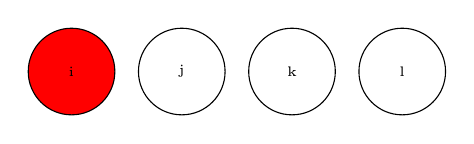
\begin{tikzpicture}
    \def\d{1.4}
    \def\size{1.1}
    \node(c1) [circle, draw, fill=red, minimum size = \size cm] at (\d * 0,0) {\tiny i};
    \node(c2) [circle, draw, minimum size = \size cm] at (\d * 1,0) {\tiny j};
    \node(c3) [circle, draw, minimum size = \size cm] at (\d * 2,0) {\tiny k};
    \node(c4) [circle, draw, minimum size = \size cm] at (\d * 3,0) {\tiny l};
\end{tikzpicture}
    \vspace{-1.7cm}
    \caption{Addition of a pawn to a position after throwing at least one six by appending an X-gate.}
    \label{fig:new_pawn}
\end{figure}

\subsection{Swap}
The swap, or direct move, happens when the same value is thrown twice. The pawn just switches positions and the circuit is a standard swap gate.
\begin{figure}[H]
    \centering
    \newsavebox{\directmovecircuit}
\newsavebox{\directmovevis}
\newsavebox{\dicedirect}

\savebox{\directmovecircuit}{
    \begin{quantikz}
        \lstick{$\ket{1}_0$} & \swap{2} & \rstick{$\ket{0}_0$}\\
        \lstick{$\ket{0}_1$}& & \rstick{$\ket{0}_1$}\\
        \lstick{$\ket{0}_2$} &\swap{-2}&\rstick{$\ket{1}_2$}\\
    \end{quantikz}
}

\savebox{\dicedirect}{
    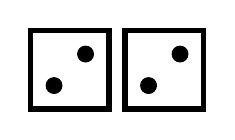
\begin{tikzpicture}
        \def\dielength{1}
        \def\dlwith{2}
        \def\dotsize{\dielength cm * 0.2}
        \node(die1) [rectangle, draw, line width = \dlwith pt, minimum width = \dielength cm, minimum height = \dielength cm] at (-\dielength/2-0.1*\dielength,0) {};
        
        \node [circle, draw, fill, minimum size = \node [circle, draw, fill, minimum size = \dotsize, inner sep=0pt] at ($(die1) + (0.2 * \dielength,0.2*\dielength)$) {};
        \node [circle, draw, fill, minimum size = \dotsize, inner sep=0pt] at ($(die1) + (-0.2 * \dielength,-0.2*\dielength)$) {};

        \node(die2) [rectangle, draw, line width = \dlwith pt, minimum width = \dielength cm, minimum height = \dielength cm] at (+\dielength/2+0.1*\dielength,0) {};
        \node [circle, draw, fill, minimum size = \node [circle, draw, fill, minimum size = \dotsize, inner sep=0pt] at ($(die2) + (0.2 * \dielength,0.2*\dielength)$) {};
        \node [circle, draw, fill, minimum size = \dotsize, inner sep=0pt] at ($(die2) + (-0.2 * \dielength,-0.2*\dielength)$) {};
    \end{tikzpicture}
}

\savebox{\directmovevis}{
    \begin{tikzpicture}
        \def\d{1.1}
        \def\size{0.8 cm}
        \node (arrow) [single arrow, draw, minimum width = 40 pt, single arrow head extend=3pt, minimum height=60 pt] at (0,0) {};
        \node (dice) [] at (0,0) {\scalebox{0.5}{\usebox{\dicedirect}}};
        
        \node (c0l) [circle, draw, minimum size = \size, pattern = horizontal lines, fill] at ($(arrow.west) + (-2.5*\d,0)$) {};
        \node[circle, fill=white, inner sep=0.3mm, text=black] at ($(arrow.west) + (-2.5*\d,0)$) {0};
        \node (c1l) [circle, draw, minimum size = \size] at ($(arrow.west) + (-1.5*\d,0)$) {1};
        \node (c2l) [circle, draw, minimum size = \size] at ($(arrow.west) + (-0.5*\d,0)$) {2};
        
        \node (c1r) [circle, draw, minimum size = \size] at ($(arrow.east) + (0.5*\d,0)$) {0};
        \node (c2r) [circle, draw, minimum size = \size] at ($(arrow.east) + (1.5*\d,0)$) {1};
        \node (c3r) [circle, draw, minimum size = \size, pattern = horizontal lines, fill] at ($(arrow.east) + (2.5*\d,0)$) {};
        \node[circle, fill=white, inner sep=0.3mm, text=black] at ($(arrow.east) + (2.5*\d,0)$) {2};
    \end{tikzpicture}
}

\begin{tikzpicture}
    \node (circuit) [] at (0,0) {\scalebox{1.5}{\usebox{\directmovecircuit}}};
    \node (vis) [above] at ($(0,0.1)+(circuit.north)$) {\usebox{\directmovevis}};
\end{tikzpicture}
    \vspace{-1.7cm}
    \caption{Swapping a pawn from a position to another position by appending a swap gate.}
    \label{fig:direct_move}
\end{figure}

\subsection{Superposition move}
When the dice have two different values, the pawn is brought in superposition. This can also be a pawn that is already in a superposition, it then splits up even more.
\begin{figure}[H]
    \centering
    \newsavebox{\superpositioncircuit}
\newsavebox{\superpositionvis}
\newsavebox{\dicesuper}

\savebox{\superpositioncircuit}{
    \begin{quantikz}
        \lstick{$\ket{1}_0$} & \ctrl{1} &\ctrl{1} & \swap{2} &           & \rstick{$\ket{0}_0$}\\[-0.5em]
        \lstick{$\ket{0}_1$} & \targ{ } &\gate{H} &          &  \ctrl{1} & \rstick[wires=2]{\begin{tabular}[t]{l} $\ket{10}_{12}$\\$-\ket{01}_{12}$\end{tabular}}\\[-0.5em]
        \lstick{$\ket{0}_2$} & &         & \swap{-2}&  \targ{ } & \\[-0.5em]
    \end{quantikz}
}

\savebox{\dicesuper}{
    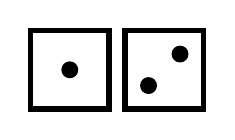
\begin{tikzpicture}
        \def\dielength{1}
        \def\dlwith{2}
        \def\dotsize{\dielength cm * 0.2}
        \node(die1) [rectangle, draw, line width = \dlwith pt, minimum width = \dielength cm, minimum height = \dielength cm] at (-\dielength/2-0.1*\dielength,0) {};
        
        \node [circle, draw, fill, minimum size = \dotsize, inner sep=0pt] at ($(die1) + (0 * \dielength,-0*\dielength)$) {};

        \node(die2) [rectangle, draw, line width = \dlwith pt, minimum width = \dielength cm, minimum height = \dielength cm] at (+\dielength/2+0.1*\dielength,0) {};
        \node [circle, draw, fill, minimum size = \dotsize, inner sep=0pt] at ($(die2) + (0.2 * \dielength,0.2*\dielength)$) {};
        \node [circle, draw, fill, minimum size = \dotsize, inner sep=0pt] at ($(die2) + (-0.2 * \dielength,-0.2*\dielength)$) {};
    \end{tikzpicture}
}

\savebox{\superpositionvis}{
    \begin{tikzpicture}
        \def\d{1.1}
        \def\size{0.8 cm}
        \node (arrow) [single arrow, draw, minimum width = 40 pt, single arrow head extend=3pt, minimum height=60 pt] at (0,0) {};
        \node (dice) [] at (0,0) {\scalebox{0.5}{\usebox{\dicesuper}}};
        \node (c0l) [circle, draw, minimum size = \size, pattern = horizontal lines, fill] at ($(arrow.west) + (-2.5*\d,0)$) {};
        \node[circle, fill=white, inner sep=0.3mm, text=black] at ($(arrow.west) + (-2.5*\d,0)$) {0};
        \node (c1l) [circle, draw, minimum size = \size] at ($(arrow.west) + (-1.5*\d,0)$) {1};
        \node (c2l) [circle, draw, minimum size = \size] at ($(arrow.west) + (-0.5*\d,0)$) {2};
        
        \node (c0r) [circle, draw, minimum size = \size] at ($(arrow.east) + (0.5*\d,0)$) {0};
        \node (c1r) [circle, draw, minimum size = \size, pattern = horizontal lines, fill, fill opacity = 0.75] at ($(arrow.east) + (1.5*\d,0)$) {};
        \node[circle, fill=white, inner sep=0.3mm, text=black] at ($(arrow.east) + (1.5*\d,0)$) {1};
        \node (c2r) [circle, draw, minimum size = \size, pattern = horizontal lines, fill, fill opacity = 0.75] at ($(arrow.east) + (2.5*\d,0)$) {};
        \node[circle, fill=white, inner sep=0.3mm, text=black] at ($(arrow.east) + (2.5*\d,0)$) {2};
    \end{tikzpicture}
}

\begin{tikzpicture}
    \node (circuit) [] at (0,0) {\scalebox{1.4}{\usebox{\superpositioncircuit}}};
    \node (vis) [above] at ($(0,0.3)+(circuit.north)$) {\usebox{\superpositionvis}};
\end{tikzpicture}
    \vspace{-1.7cm}
    \caption{A classical pawn that goes into superposition by appending the superposition circuit. The amplitudes are not normalized.}
    \label{fig:superposition_move}
\end{figure}

\subsection{Capture}
When a pawn lands on top of a pawn of a different colour, the original pawn is captured. The capturing circuit in itself is just a controlled not gate, where the controlling qubits is the capturing pawn \textit{and} all the inverted qubits the captive is in superposition with. \\
The capturing pawn does not go to the position of the captive (due to the no double occupancies rule), but goes to the next available position. This could be the position right after the captive, or could be any amount of positions after it. It does not capture the pawns on the way of finding a new position. This is also included in the example of Figure \ref{fig:capture_move}.
\begin{figure}[H]
    \centering
    \newsavebox{\capturecircuit}
\newsavebox{\capturevis}
\newsavebox{\dicecapture}

\savebox{\capturecircuit}{
    \begin{quantikz}
        \lstick{$\ket{1}_0$} & \swap{3}  &&          && \rstick{$\ket{0}_0$}\\[-0.5em]
        \lstick[wires=2]{\begin{tabular}[t]{r} $\ket{10}_{12}$\\$+\ket{01}_{12}$\end{tabular}} &  &\gategroup[3,steps=3,style={inner
sep=1pt}, label style={label position=below,anchor=north,yshift=-0.2cm}]{capturing circuit}& \targ{ } && \rstick[wires=2]{\begin{tabular}[t]{l} $\ket{00}_{12}$\\$+\ket{01}_{12}$\end{tabular}}\\[-0.5em]
                             &           &\gate{X} & \ctrl{-1}&\gate{X}&   \\[-0.5em]
        \lstick{$\ket{0}_3$} & \swap{-3} && \ctrl{-2}&& \rstick{$\ket{1}_3$}
    \end{quantikz}
}

\savebox{\dicecapture}{
    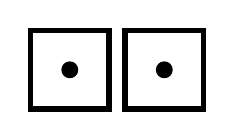
\begin{tikzpicture}
        \def\dielength{1}
        \def\dlwith{2}
        \def\dotsize{\dielength cm * 0.2}
        \node(die1) [rectangle, draw, line width = \dlwith pt, minimum width = \dielength cm, minimum height = \dielength cm] at (-\dielength/2-0.1*\dielength,0) {};
        
        \node [circle, draw, fill, minimum size = \dotsize, inner sep=0pt] at ($(die1) + (0 * \dielength,-0*\dielength)$) {};

        \node(die2) [rectangle, draw, line width = \dlwith pt, minimum width = \dielength cm, minimum height = \dielength cm] at (+\dielength/2+0.1*\dielength,0) {};
        \node [circle, draw, fill, minimum size = \dotsize, inner sep=0pt] at ($(die2) + (0 * \dielength,0*\dielength)$) {};
    \end{tikzpicture}
}

\savebox{\capturevis}{
    \begin{tikzpicture}
        \def\d{1.1}
        \def\size{0.8 cm}
        \node (arrow) [single arrow, draw, minimum width = 40 pt, single arrow head extend=3pt, minimum height=60 pt] at (0,0) {};
        \node (dice) [] at (0,0) {\scalebox{0.5}{\usebox{\dicecapture}}};
        \node (c0l) [circle, draw, minimum size = \size, pattern = horizontal lines, fill] at ($(arrow.west) + (-2.5*\d,0)$) {};
        \node[circle, fill=white, inner sep=0.3mm, text=black] at ($(arrow.west) + (-2.5*\d,0)$) {0};
        \node (c1l) [circle, draw, minimum size = \size, pattern = crosshatch dots, fill, fill opacity = 0.75] at ($(arrow.west) + (-1.5*\d,0)$) {};
        \node[circle, fill=white, inner sep=0.3mm, text=black] at (c1l) {1};
        \node (c2l) [circle, draw, minimum size = \size, pattern = crosshatch dots, fill, fill opacity = 0.75] at ($(arrow.west) + (-0.5*\d,0)$) {2};
        \node[circle, fill=white, inner sep=0.3mm, text=black] at (c2l) {2};
        
        \node (c1r) [circle, draw, minimum size = \size, pattern = crosshatch dots, fill, fill opacity = 0.75] at ($(arrow.east) + (0.5*\d,0)$) {};
        \node[circle, fill=white, inner sep=0.3mm, text=black] at (c1r) {1};
        \node (c2r) [circle, draw, minimum size = \size, pattern = crosshatch dots, fill, fill opacity = 0.75] at ($(arrow.east) + (1.5*\d,0)$) {};
        \node[circle, fill=white, inner sep=0.3mm, text=black] at (c2r) {2};
        \node (c3r) [circle, draw, minimum size = \size, pattern = horizontal lines, fill, fill opacity = 0.75] at ($(arrow.east) + (2.5*\d,0)$) {};
        \node[circle, fill=white, inner sep=0.3mm, text=black] at (c3r) {3};
    \end{tikzpicture}
}

\begin{tikzpicture}
    \node (circuit) [] at (0,0) {\scalebox{1.2}{\usebox{\capturecircuit}}};
    \node (vis) [above] at ($(0,0.3)+(circuit.north)$) {\usebox{\capturevis}};
\end{tikzpicture}
    \vspace{-0.9cm}
    \caption{Capturing a pawn in a superposition using a swap move. The swap gate is \textit{not} part of the capturing circuit. Even though the moving pawn should go to position 1, it goes the next free position, which is position 3. It does not capture pawn 2 when moving to the next free position.}
    \label{fig:capture_move}
\end{figure}

\subsection{Measure}
The circuit is measured when a pawn enters its final position, or when the total number of occupied positions (by any pawn) exceeds twenty. The measurements happen for all the pawns at the same time. The measurement bases are dependent on the colour of the pawn that reaches the winning position. 

\begin{figure}[H]
    \centering
    \newsavebox{\measurecircuit}
\newsavebox{\measurevis}


\savebox{\measurecircuit}{
    \begin{quantikz}
        \lstick[wires=2]{\begin{tabular}[t]{r} $\ket{10}_{01}$\\$+\ket{01}_{01}$\end{tabular}} & \meter{}  & \setwiretype{c} \\[-0.5em]
        & \meter{} & \setwiretype{c} \\[-0.5em]
    \end{quantikz}
}

\savebox{\measurevis}{
    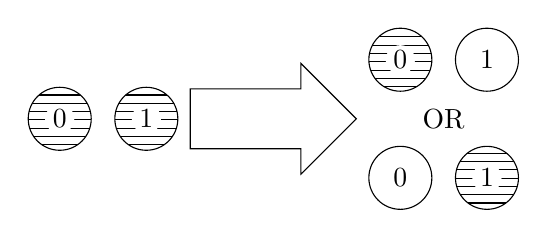
\begin{tikzpicture}
        \def\d{1.1}
        \def\size{0.8 cm}
        \node (arrow) [single arrow, draw, minimum width = 40 pt, single arrow head extend=3pt, minimum height=60 pt] at (0,0) {};
        \node (c0l) [circle, draw, minimum size = \size, pattern = horizontal lines, fill, fill opacity=0.75] at ($(arrow.west) + (-1.5*\d,0)$) {};
        \node[circle, fill=white, inner sep=0.3mm, text=black] at (c0l) {0};
        \node (c1l) [circle, draw, minimum size = \size, pattern = horizontal lines, fill, fill opacity = 0.75] at ($(arrow.west) + (-0.5*\d,0)$) {};
        \node[circle, fill=white, inner sep=0.3mm, text=black] at (c1l) {1};

        \def\h{0.75}
        
        \node (c0ar) [circle, draw, minimum size = \size, pattern = horizontal lines, fill, fill opacity = 0.75] at ($(arrow.east) + (0.5*\d,\h)$) {};
        \node[circle, fill=white, inner sep=0.3mm, text=black] at (c0ar) {0};
        \node (c1ar) [circle, draw, minimum size = \size] at ($(arrow.east) + (1.5*\d,\h)$) {1};

        \node [] at ($(arrow.east) + (1*\d,0)$) {OR};
        
        \node (c0br) [circle, draw, minimum size = \size] at ($(arrow.east) + (0.5*\d,-\h)$) {0};
        \node (c1br) [circle, draw, minimum size = \size, pattern = horizontal lines, fill, fill opacity = 0.75] at ($(arrow.east) + (1.5*\d,-\h)$) {};
        \node[circle, fill=white, inner sep=0.3mm, text=black] at (c1br) {1};
    \end{tikzpicture}
}

\begin{tikzpicture}
    \node (circuit) [] at (0,0) {\scalebox{1.5}{\usebox{\measurecircuit}}};
    \node (vis) [above] at ($(0,0.3)+(circuit.north)$) {\usebox{\measurevis}};
\end{tikzpicture}
    \vspace{-0.9cm}
    \caption{Measuring a circuit in the Z-basis that describes one pawn in a single superposition, which updates the game accordingly: the pawn collapses into the first or the second position.}
    \label{fig:measure_move}
\end{figure}


\section{Code}\label{QuantumCode}

%% If you have bibdatabase file and want bibtex to generate the
%% bibitems, please use
%%

For all code references, please visit the GitHub repository at [\url{https://github.com/SjdTl/QuantumEngineering}]. The README file contains contains instructions to run the game, high-level documentation and some example pictures of the game.  A video walk-through of the game can also be found on \href{https://www.youtube.com/watch?v=1wOmJI2PlPA}{\color{red}YouTube} \cite{youtubewalkthrough}.

%% else use the following coding to input the bibitems directly in the
%% TeX file.

% \begin{thebibliography}{00}

% \bibitem[Author(year)]{label}
% % For example:
% \bibitem[Aladro et al.(2015)]{Aladro15} Aladro, R., Martín, S., Riquelme, D., et al. 2015, \aas, 579, A101

% \end{thebibliography}

\printbibliography

\end{document}

\endinput
%%
%% End of file `elsarticle-template-harv.tex'.
